\section{Reducing the rank of a surface diagram}
\label{sec:reduction}

We prove the nonclosed step in the diagram-density induction.  Call a
diagram \emph{normalized} if all its facets have positive rank and every
seam has at least two children; call these seams \emph{proper}.
The first subsection explains how to reach this form.  This operation
may create closed facets, so it must precede their separation from the
facets with boundary.

\begin{proposition}\label{prop:nonclosed-reduction}
Let $2\leq n\leq r$, and suppose integral solutions are dense for every
surface diagram of ranks less than $n$.  Then they are dense for every
normalized diagram of ranks at most $n$ whose rank-$n$ facets have
nonempty boundary.  Closed facets of smaller rank are allowed.
\end{proposition}

We prove the proposition by constructing finitely many lower-rank
diagrams from which every original solution can be recovered.  Over
each lower solution variety, reconstruction consists of successive
locally affine bundles and changes of frames.  Every integral lower
solution admits lifts, with dense integral choices in each fiber.
Lemma~\ref{lem:density-transfer} will then give the conclusion.

There are two geometric stages.  First, removing bands cuts the
rank-$n$ facets to disks; the two-flag lemma recovers each band through
affine matching choices.  Next, a proper subspace and its quotient
replace each disk.  The vertex constructions ensure that arbitrary
lower data admit the successive lifts needed to reconstruct the disk,
including closure around its boundary.

\subsection{Removing identity seams}
\label{subsec:identity-normalization}

Delete every zero-rank facet and every zero child.  Interchanges with
a zero child become continuations.  A seam with one positive child
is an \emph{identity seam}; its specified isomorphism sews its two
sides together.  Opposite boundary orientations give an oriented
surface.  At a split vertex with only one positive subblock, this
sewing turns the split into continuation.  If the original parent
list has just one positive block, sewing identifies its refined
list with the additional seam.  If all three lists have one positive
block, three corner sectors sew to a disk, and the refinement
compatibility is precisely the composition condition for the local
system to extend over its center.  Identity circle seams are sewn
in the same way.

These operations use occurrences of boundary germs and therefore also
apply to seams incident several times to the same facet.  Solutions
of the sewn diagram restrict to solutions of the old one; allowing
frame changes gives all old solutions.  The construction is valid
over $R$.  We can consequently work with normalized diagrams.
A facet of maximal rank $n$ can then only be a parent, and
every child on its boundary has rank less than $n$.

The closed rank-$n$ facets of a normalized diagram are independent
factors of its solution variety.  Set them aside when applying
Proposition~\ref{prop:nonclosed-reduction}; Sections~\ref{sec:surfaces}
and~\ref{sec:dynamics} will supply their density.  We now prove the
proposition for the remaining diagram, using only the smaller-rank
induction hypothesis.  If it has no rank-$n$ facets, that hypothesis
already applies.

\subsection{Cutting the maximal-rank facets to disks}

In each nonclosed rank-$n$ facet choose disjoint properly embedded
arcs which cut the underlying surface to disks.  Their endpoints are
distinct interior points of seam intervals; an unmarked circle seam
may first be marked.  The arcs avoid all punctures, which do not
affect this topological choice.  Remove narrow bands around the arcs.

Consider one band.  At its two short ends, the old seams give flags
of types $F_\bullet$ and $H_\bullet$.  On each long side put the
two-flag sequence of Lemma~\ref{lem:two-flags}, with the same array
of block ranks on the two sides.  Across the band put a lower-rank
strip for each block of the running list.  Its two long sides are
children of the two parent sides.  At a short end it extends the
corresponding old child facet.  To split a block on both long sides,
put a transverse seam across its strip; its endpoints give the two
split vertices.  Merges reverse this construction.  At an
interchange put an interchange vertex on both parents and continue
each labeled strip unchanged.  Strips may cross one another in this
description: the diagram is specified by its side incidences, not
by a planar embedding.
Figure~\ref{fig:band-gallery} shows one strip occurrence and the
two-by-two example of the common gallery; its blocks $W_{ij}$ have
ranks $m_{ij}$.

\begin{figure}[ht]
\centering
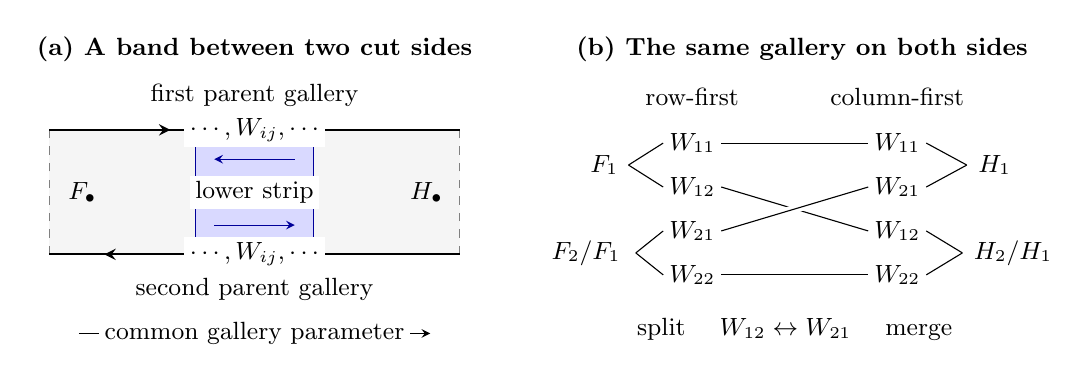
\begin{tikzpicture}[x=.93cm,y=.93cm,>=stealth,
  every node/.style={font=\small},
  block/.style={fill=white,inner sep=2pt}]
  \node[font=\small\bfseries] at (2.8,2.8) {(a) A band between two cut sides};
  \fill[gray!8] (0,0) rectangle (5.6,1.7);
  \draw[dashed,gray] (0,0)--(0,1.7) (5.6,0)--(5.6,1.7);
  \fill[blue!15] (2.0,0) rectangle (3.6,1.7);
  \draw[blue!60!black] (2.0,0)--(2.0,1.7) (3.6,0)--(3.6,1.7);
  \draw[thick] (0,1.7)--(5.6,1.7) (0,0)--(5.6,0);
  \draw[->,thick] (.75,1.7)--(1.65,1.7);
  \draw[<-,thick] (.75,0)--(1.65,0);
  \draw[<-,blue!60!black] (2.25,1.3)--(3.35,1.3);
  \draw[->,blue!60!black] (2.25,.4)--(3.35,.4);
  \node[block] at (2.8,1.7) {$\cdots,W_{ij},\cdots$};
  \node[block] at (2.8,0) {$\cdots,W_{ij},\cdots$};
  \node at (2.8,2.17) {first parent gallery};
  \node at (2.8,-.47) {second parent gallery};
  \node at (.45,.85) {$F_\bullet$};
  \node at (5.15,.85) {$H_\bullet$};
  \node[align=center,fill=white,inner sep=2pt] at (2.8,.85)
       {lower strip};
  \draw[->] (.4,-1.08)--(5.2,-1.08);
  \node[fill=white,inner sep=2pt] at (2.8,-1.08)
       {common gallery parameter};

  \begin{scope}[xshift=7.0cm]
    \node[font=\small\bfseries] at (2.75,2.8) {(b) The same gallery on both sides};
    \node at (.05,1.22) {$F_1$};
    \node at (-.2,.02) {$F_2/F_1$};
    \node[block] (l11) at (1.25,1.52) {$W_{11}$};
    \node[block] (l12) at (1.25,.92) {$W_{12}$};
    \node[block] (l21) at (1.25,.32) {$W_{21}$};
    \node[block] (l22) at (1.25,-.28) {$W_{22}$};
    \node[block] (r11) at (4.05,1.52) {$W_{11}$};
    \node[block] (r21) at (4.05,.92) {$W_{21}$};
    \node[block] (r12) at (4.05,.32) {$W_{12}$};
    \node[block] (r22) at (4.05,-.28) {$W_{22}$};
    \node at (5.38,1.22) {$H_1$};
    \node at (5.63,.02) {$H_2/H_1$};
    \draw (.38,1.22)--(l11.west) (.38,1.22)--(l12.west);
    \draw (.48,.02)--(l21.west) (.48,.02)--(l22.west);
    \draw (l11.east)--(r11.west) (l22.east)--(r22.west);
    \draw (l12.east)--(r12.west);
    \draw[preaction={draw=white,line width=3pt}]
          (l21.east)--(r21.west);
    \draw (r11.east)--(5.0,1.22) (r21.east)--(5.0,1.22);
    \draw (r12.east)--(4.94,.02) (r22.east)--(4.94,.02);
    \node at (1.25,2.15) {row-first};
    \node at (4.05,2.15) {column-first};
    \node[align=center] at (2.65,-1.02)
      {split\quad\ $W_{12}\leftrightarrow W_{21}$\quad\ merge};
  \end{scope}
\end{tikzpicture}

\caption{Replacing a cut band by lower-rank strips.
Both parent sides carry the same gallery from $F_\bullet$ to
$H_\bullet$, with the same array $(m_{ij})$.
Panel (a) displays one strip occurrence; the arrows on its boundary
oppose the parent boundary arrows.  The galleries use a common
parameter, independently of those boundary orientations.
Panel (b) shows the two-by-two sorting pattern, with $F_2=H_2=V$.
Splits and merges
are performed on both parent sides, using transverse seams on the
relevant strips.  The crossing represents an interchange and adds
no incidence between strips.  This is an incidence schematic,
not a planar embedding of the whole diagram.}
\label{fig:band-gallery}
\end{figure}

All strips inherit the band orientation.  Their long-side boundary
orientations are opposite to those of the corresponding parents,
and the short-end attachments sew opposite orientations.  Thus the
result is again an oriented surface diagram.  Its only rank-$n$
facets are disks, possibly with punctures.  Every new strip has rank
less than $n$, since it refines a child of a proper seam.  Zero
blocks can be deleted.

We verify reconstruction before applying density.  A solution of
the cut diagram gives two pairs of flags, one on each side of the
band.  The old child transports prescribe isomorphisms on their
$F$-graded and $H$-graded modules.  Transverse split and merge seams
make those isomorphisms preserve the refinements.  Transports on the
fully refined strips and the natural maps at interchanges make
them agree on the double-graded modules.  Lemma~\ref{lem:two-flags}
therefore supplies a full isomorphism respecting the entire gallery,
not just its endpoint flags.  Use it to sew back
the rank-$n$ band.  The old seam flags extend across its short ends.
Different bands give independent matching choices.

Conversely, transport the two endpoint flags of an old solution
into a band.  Their intersection ranks specify one of finitely many
arrays; a simultaneous splitting gives its two-flag sequences and
all the strips, matched by the old band transport.  This produces
a cut solution reconstructing the old one.  The matching choices
form locally affine bundles by Lemma~\ref{lem:two-flags}, and over
integral cut solutions they have dense integral parameters.  Thus
Lemma~\ref{lem:density-transfer} reduces the problem to diagrams
whose maximal-rank facets are disks.  The added topology of the
lower-rank facets is retained and causes no restriction in the
induction hypothesis.

\subsection{Replacing a disk by a subspace and a quotient}

Let $V$ be one rank-$n$ disk.  At one starting boundary interval,
choose a nonzero proper prefix of its seam flag, ending at index $k$.
Such a prefix exists because the seam is proper.  In an old solution
this subspace extends to a parallel subsystem $U$ throughout the
punctured disk, because every puncture monodromy is scalar.  Put
$Q=V/U$.  Both ranks are less than $n$, and both systems have the
same scalar puncture monodromies as $V$.

The prefix will make the reconstruction close around the boundary.
At this interval the induced flags satisfy $Q_i=0$ for $i\leq k$
and $U_i=U$ for $i\geq k$.  Once these flags and their identified
quotients are fixed, they have a unique lift in $U\oplus Q$: before
$k$ it is the given flag in $U$, and after $k$ it is the inverse
image of the flag in $Q$.  Equivalently, the stabilizer in
Lemma~\ref{lem:filtered-lift} is all of $H=\Hom(Q,U)$.
These zero-rank conditions will be part of the chosen lower diagram,
so the unique starting lift exists for every lower solution, not only
for one extracted from an old solution.

On an interval with old seam list $W_1,\ldots,W_m$, the old flag
induces flags on $U,Q$ and exact sequences
\begin{equation}\label{eq:boundary-exact-sequences}
 0\longrightarrow U_i/U_{i-1}\longrightarrow W_i
 \longrightarrow Q_i/Q_{i-1}\longrightarrow0.
\end{equation}
Choose the ranks of all these modules, and of the modules at the
finitely many vertices below.  There are finitely many possibilities;
we use the possibilities arising from old complex solutions.  The
actual construction of the lower diagram depends only on these
ranks, not on the old solution.  In particular, at the starting
interval the $Q$-graded pieces have rank zero for $i\leq k$, and the
$U$-graded pieces have rank zero for $i>k$.
Intersections and projection images are extracted only from complex
solutions.  Integral reconstruction will instead use the specified
free child modules; it does not require intersections of arbitrary
$R$-lattices to be free.

Replace $V$ by two disks $U,Q$, with the same orientation and scalar
punctures.  On a regular interval replace its seam by
\[
 U:(u_1,\ldots,u_m),\qquad
 Q:(q_1,\ldots,q_m),\qquad
 W_i:(u_i,q_i).
\]
Here $u_i$ is an actual strip joining the $U$ side to the $W_i$
side, as child on both, and $q_i$ similarly joins $Q$ to $W_i$.
Its transport gives the maps in
\eqref{eq:boundary-exact-sequences}.  Along an unmarked seam circle
these may be cyclic strips.  The old parent and child have opposite
boundary orientations, so the strips sew with the required
orientations.

We describe the two vertex replacements.  In these descriptions,
time increases along the positive boundary orientation of $V$, and
along those of $U,Q$.  It therefore runs opposite to the old child
boundary orientation.  Unaffected strips and lists continue.

Each replacement has a common reconstruction requirement.  At a split,
the coarse quotient is $W$ with its internal flag; at an interchange,
it is $A\oplus B$ with its given decomposition.  The lower data must
supply an exact sequence with this middle term whose restrictions
are the exact data on both neighboring intervals.
Lemma~\ref{lem:filtered-lift} will then extend an incoming interval
lift to the vertex, and that choice will determine the outgoing lift.

\subsubsection*{A split or merge}

Suppose an old block $W$ splits into $W'_1,\ldots,W'_s$.  Before
the event its list is $W:(w,q)$.  Split the $w,q$ connections into
$w_1,\ldots,w_s$ and $q_1,\ldots,q_s$ by transverse seams, refining
the lists at both ends of each connection.  On $W$, use the
two-flag sequence to interleave them as
\[
 w_1,q_1,\ldots,w_s,q_s.
\]
Merge each pair in this list to $W'_j$, introducing the side of
$W'_j$ through the merge vertex and its seam $W'_j:(w_j,q_j)$.
The resulting list on $W$ continues onto the old additional seam
$W:(W'_1,\ldots,W'_s)$.

At this merge vertex the $W'_j$ corner joins its occurrence as a
child of $W$ to its occurrence as parent of $w_j,q_j$.  The strip
boundaries formerly at $W$ continue at $W'_j$, and their other ends
remain at $U,Q$.  This describes all germ pairings.  The $W$ lists
run opposite to its boundary orientation toward the old side seam;
the $W'_j$ sides run into that seam as children and out along their
new strips as parents.  Hence the orientations agree.  Reverse
this construction for an old merge.

Lemma~\ref{lem:two-flags} says exactly what the construction records:
the flag of $W$ with two pieces $w,q$ is compared with its flag
having pieces $W'_j$.  Their intersections induce the refined flags
on $U,Q$, and the matched double-graded maps give the exact sequences
for the $W'_j$.  Every old complex solution admits this replacement.
Conversely, any lower solution supplies these compatible refined
exact sequences, including all their identified quotients.

Here the seam $W:(w,q)$ supplies the coarse exact sequence, and the
retained seam $W:(W'_1,\ldots,W'_s)$ supplies its internal flag.
The two-flag gallery makes their induced fine quotient maps agree.
Thus every lower solution supplies the coarse exact sequence with
middle term $W$ and its fixed internal flag, not only the sequences on
the fine quotients $W'_j$.  The restriction of a vertex lift to the coarse
interval is the identity.  On the fine interval we forget the full
identification with $W$.  For the exact sequences
$0\to w_j\to W'_j\to q_j\to0$, free compatible splittings give
\[
 K_{\rm interval}/K_{\rm coarse}
     =\bigoplus_{k<j}\Hom_R(q_j,w_k).
\]
The restriction to that interval is therefore an affine surjection
with free integral parameters.  The same two restrictions handle the
reverse merge.

\subsubsection*{An interchange and the negative scalar}

Now suppose the old event interchanges $A,B$.  Their coarsened
quotient of $V$ is identified with $A\oplus B$.  In an old solution
write $U_*\subset A\oplus B$ and $Q_*=(A\oplus B)/U_*$ for the
induced subquotients.  Put
\[
 a=U_*\cap A,\quad b=U_*\cap B,\quad
 \widetilde a=\operatorname{pr}_A(U_*),\quad
 \widetilde b=\operatorname{pr}_B(U_*).
\]
The modules $\widetilde a/a$ and $\widetilde b/b$ have the same rank,
denoted $h$.  Put $x=A/\widetilde a$ and $y=B/\widetilde b$.
The required before and after lists are
\[
\begin{array}{c|cc}
 &\text{before}&\text{after}\\ \hline
 U_*&a,\widetilde b&b,\widetilde a\\
 Q_*&A/a,y&B/b,x\\
 A&a,A/a&\widetilde a,x\\
 B&\widetilde b,y&b,B/b.
\end{array}
\]
These symbols name ranks and strip occurrences in the new diagram;
the intersection description explains how every old solution
determines such data.

Split the incoming $\widetilde b$ connection into $b,h$, and the
incoming $A/a$ connection into $h,x$.  The four lists become
\[
 U_*:(a,b,h),\quad Q_*:(h,x,y),\quad
 A:(a,h,x),\quad B:(b,h,y).
\]
Interchange $a,b$ on $U$ and $x,y$ on $Q$, leaving those connections
unchanged.  Replace the two $h$ connections
\[
 (U,B),(Q,A)\qquad\text{by}\qquad(U,A),(Q,B)
\]
using one punctured disk of rank $h$, with scalar monodromy $-I$.
Its boundary contacts, all as child, occur in the cyclic order
$U,B,Q,A$.  Along $U$ it runs from positive to negative time,
then crosses the incoming $(U,B)$ strip end; along $B$ it runs
from negative to positive time, then crosses the outgoing $(B,Q)$
end; along $Q$ it runs from positive to negative time, then crosses
the incoming $(Q,A)$ end; along $A$ it runs from negative to positive
time, then crosses the outgoing $(A,U)$ end.  This specifies the
oriented sewing to all four strip ends.  Finally merge $a,h$ to
$\widetilde a$ and $h,y$ to $B/b$.  If $h=0$, delete this disk.

The lower solution provides maps $p_A:U_*\to A$, $p_B:U_*\to B$,
$i_A:A\to Q_*$ and $i_B:B\to Q_*$, with the images and kernels
specified in the table.  Write
\[
 h_U=U_*/(a\oplus b),\qquad
 h_A=\widetilde a/a,\qquad h_B=\widetilde b/b,\qquad
 h_Q=\operatorname{im}i_A\cap\operatorname{im}i_B.
\]
These are the rank-$h$ subquotients at the four contacts.  The maps
$p_A,p_B$ induce isomorphisms from $h_U$ to $h_A,h_B$, and
$i_A,i_B$ induce isomorphisms from $h_A,h_B$ to $h_Q$.
Figure~\ref{fig:swap-disk} displays the two resulting paths from
$h_U$ to $h_Q$.

\begin{figure}[ht]
\centering
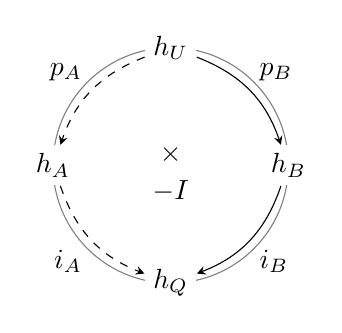
\begin{tikzpicture}[scale=1.15,>=stealth]
  \draw[gray] (0,0) circle (1.3);
  \node[fill=white,inner sep=3pt] (u) at (0,1.3) {$h_U$};
  \node[fill=white,inner sep=3pt] (b) at (1.3,0) {$h_B$};
  \node[fill=white,inner sep=3pt] (q) at (0,-1.3) {$h_Q$};
  \node[fill=white,inner sep=3pt] (a) at (-1.3,0) {$h_A$};
  \draw[->] (u) to[bend left=25] node[above right] {$p_B$} (b);
  \draw[->] (b) to[bend left=25] node[below right] {$i_B$} (q);
  \draw[->,dashed] (u) to[bend right=25] node[above left] {$p_A$} (a);
  \draw[->,dashed] (a) to[bend right=25] node[below left] {$i_A$} (q);
  \node at (0,0.12) {$\times$};
  \node at (0,-0.28) {$-I$};
\end{tikzpicture}

\caption{The four contacts of the punctured $h$-disk.
The symbols denote the corresponding $h$-subquotients and the
maps they inherit.  The two paths from $h_U$ to $h_Q$ differ by
the monodromy $-I$, so $i_Ap_A+i_Bp_B=0$.}
\label{fig:swap-disk}
\end{figure}

The two composites $i_Ap_A,i_Bp_B$ factor through $h_U$ to $h_Q$.
They are opposite, because they are the two transports around the
punctured $h$-disk.  Hence the following sequence is a complex:
\begin{equation}\label{eq:swap-exact-sequence}
 0\longrightarrow U_*
 \xrightarrow{(p_A,p_B)}A\oplus B
 \xrightarrow{(i_A,i_B)}Q_*\longrightarrow0
\end{equation}
It is exact over $R$ as well as over $\C$.  The kernels of $p_A,p_B$
are respectively $b,a$, and their intersection is zero by the
interchange on $U$.  The images of $i_A,i_B$ span $Q_*$ because
their $x,y$ quotients are complementary.  If
$i_A(z)+i_B(t)=0$, projection modulo $\operatorname{im}i_A$ gives
$t\in\widetilde b$.  Lift $t$ under $p_B$ and subtract the image
of that lift; the remaining vector is in $\ker i_A=a$, which is
again in the image of $U_*$.  The needed lifts exist over $R$
because the named quotients are free.

For clarity, in split coordinates the maps are
\begin{align*}
 U_*&=a\oplus b\oplus h,&A&=a\oplus h\oplus x,\\
 Q_*&=h\oplus x\oplus y,&B&=b\oplus h\oplus y,\\
 p_A(a,b,h)&=(a,h,0),&p_B(a,b,h)&=(b,h,0),\\
 i_A(a,h,x)&=(h,x,0),&i_B(b,h,y)&=(-h,0,y).
\end{align*}
Thus the scalar $-I$ supplies exactly the sign needed in
\eqref{eq:swap-exact-sequence}; no division by $2$ is involved.
Conversely, any old exact sequence with the induced flags gives
the refinements and maps above, and its two induced $h$-maps have
this opposite sign.  They therefore extend over the punctured disk.

The exact sequence with middle term $A\oplus B$ is the coarse vertex
data required for reconstruction.  In the displayed free coordinates,
forgetting its full identification permits the additional stabilizer
block $\Hom_R(y,a)$ on the incoming interval and $\Hom_R(x,b)$ on
the outgoing interval.  All unchanged blocks cancel from these
quotients.  Each restriction is considered separately: split its
refined flags on $U,Q$ and group the free summands to obtain the
coarse flags.  Both restrictions are affine surjections with free
integral parameters.  No simultaneous choice of both interval lifts
is required.

All replacements occur in separate side intervals and corner
neighborhoods.  They preserve the other seams of every lower-rank
facet, including repeated occurrences of the same facet.  Parallel
maps on the strips extend across the specified cross sections, so
the construction also applies to cyclic boundary lists.

\subsection{Reconstruction and closure around a disk}

We now reconstruct a disk from an arbitrary solution of its lower
diagram.  Put $V=U\oplus Q$.  All puncture monodromies are the
prescribed scalars, so this is a local system with the required
monodromy.  Moreover $H=\Hom(Q,U)$ is constant on the punctured
disk: the identical scalar monodromies of $U,Q$ act trivially on it.

The starting interval has the unique lift already established.
Continue it by parallel transport to the first vertex.  The relevant
vertex construction gives an affine space of extensions of this
incoming lift.  Choose one and restrict it to the outgoing interval,
then repeat around the boundary.  Every step is surjective with affine
fiber, and over integral lower data that fiber has free integral
parameters.  On return, the starting interval still has just one lift,
so the propagated lift agrees with it automatically.  This includes
all identified quotients: they belong to the lift spaces and are not
additional data to be matched afterward.  With no vertices, the same
unique lift is parallel around the unmarked seam circle.  Thus closure
imposes no further equation.

For each fixed rank pattern these successive choices form a finite
tower of locally affine bundles over the lower solution variety.
Indeed the flags have constant ranks, so they can be split locally,
and the preceding matrix-block descriptions give each event fiber.
Every integral lower solution admits integral choices, dense in those
fibers by Lemma~\ref{lem:integral-parameters}.  Conversely, every old
complex solution is recovered from its induced lower data and its
original lifts, up to the allowed frame changes.  Its disk local
system is isomorphic to $U\oplus Q$ because all puncture generators
act by the prescribed scalars.

Perform the construction on every rank-$n$ disk.  No new rank-$n$
facet has been introduced.  After normalizing zero blocks and
identity seams, the induction hypothesis gives density on each
resulting lower diagram.  Lemma~\ref{lem:density-transfer} gives
density on the disk diagrams and then on the original nonclosed
diagram.  This proves Proposition~\ref{prop:nonclosed-reduction}.

Closed maximal-rank facets remain.  The next two sections treat their
scalar-monodromy equations; after the closed-density lemma we assemble
the full induction proving Theorem~\ref{thm:diagram-density}.
